\documentclass[11pt,letterpaper]{article}
\usepackage[lmargin=1in,rmargin=1in,tmargin=1in,bmargin=1in]{geometry}
\usepackage{../style/homework}
\usepackage{../style/commands}
\setbool{quotetype}{false} % True: Side; False: Under
\setbool{hideans}{true} % Student: True; Instructor: False

% -------------------
% Content
% -------------------
\begin{document}

\homework{13: Due 01/13}{It has been said that geometry is the art of applying good reasoning to bad diagrams.}{Richard J. Trudeau}

% Problem 1
\problem{10} Find the degrees of each vertex in the graph below and find the degree of the graph.
	\[
	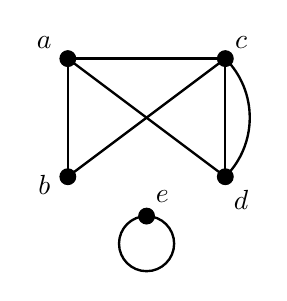
\begin{tikzpicture}
	\draw[line width=0.03cm] (0,0) -- (0,1.5) -- (2,1.5) -- (2,0);
	\draw[line width=0.03cm] (0,1.5) -- (2,0);
	\draw[line width=0.03cm] (0,0) -- (2,1.5);
	\draw[line width=0.03cm] (2,0) to[out= 45,in= -45] (2,1.5);
	\draw[line width=0.03cm] (1,-0.85) circle (0.35); 
	
	\draw[fill=black] (0,0) circle (0.1); 
	\draw[fill=black] (2,0) circle (0.1); 
	\draw[fill=black] (2,1.5) circle (0.1); 
	\draw[fill=black] (0,1.5) circle (0.1); 
	\draw[fill=black] (1,-0.5) circle (0.1); 
	
	\node at (-0.3,1.7) {$a$};
	\node at (-0.3,-0.1) {$b$};
	\node at (2.2,1.7) {$c$};
	\node at (2.2,-0.3) {$d$};
	\node at (1.2,-0.25) {$e$};
	\end{tikzpicture}
	\]



\newpage



% Problem 2
\problem{10} Find the in- and out-degree of each vertex in the graph below:
	\[
	\begin{tikzpicture}
	\begin{scope}[very thick,decoration={
	markings,
	mark=at position 0.5 with {\arrow{>}}
				}
	] 
	\draw[line width=0.03cm,postaction={decorate}] (0,2) -- (0,0);
	\draw[line width=0.03cm,postaction={decorate}] (0,2) -- (2,2);
	\draw[line width=0.03cm,postaction={decorate}] (2,2) -- (2,0);
	\draw[line width=0.03cm,postaction={decorate}] (2,0) -- (0,2);
	\draw[line width=0.03cm,domain=90:270,->] plot ({0.433*cos(\x)}, {-0.433+0.433*sin(\x)});
	\draw[line width=0.03cm,domain=-90:90] plot ({0.433*cos(\x)}, {-0.433+0.433*sin(\x)});

	\draw[fill=black] (0,0) circle (0.1); 
	\draw[fill=black] (0,2) circle (0.1); 
	\draw[fill=black] (2,2) circle (0.1); 
	\draw[fill=black] (2,0) circle (0.1); 
	
	\node at (-0.3,2.2) {$a$};
	\node at (2.3,2.2) {$b$};
	\node at (-0.3,0.2) {$c$};
	\node at (2.3,0.2) {$d$};
	\end{scope}
	\end{tikzpicture}
	\]



\newpage



% Problem 3
\problem{10} Does the graph below have an Euler circuit or an Euler trail? Explain. If it has either, find it. 
	\[
	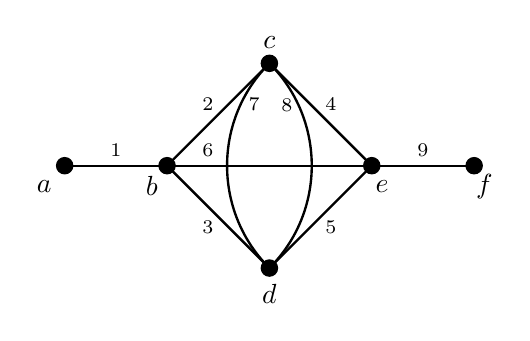
\begin{tikzpicture}[scale=1.3]
	\draw[line width=0.03cm] (0,0) -- (4,0);
	\draw[line width=0.03cm] (1,0) -- (2,1) -- (3,0) -- (2,-1) -- (1,0);
	\draw[line width=0.03cm] (2,-1) to[out= 45,in= -45] (2,1);
	\draw[line width=0.03cm] (2,-1) to[out= 135,in= -135] (2,1);
	
	\draw[fill=black] (0,0) circle (0.08); 
	\draw[fill=black] (1,0) circle (0.08); 
	\draw[fill=black] (2,1) circle (0.08); 
	\draw[fill=black] (2,-1) circle (0.08); 
	\draw[fill=black] (3,0) circle (0.08); 
	\draw[fill=black] (4,0) circle (0.08); 
	
	\node at (-0.2,-0.2) {$a$};
	\node at (0.85,-0.2) {$b$};
	\node at (2,1.2) {$c$};
	\node at (2,-1.25) {$d$};
	\node at (3.1,-0.2) {$e$};
	\node at (4.1,-0.2) {$f$};
	
	\node at (0.5,0.15) {\scriptsize$1$};
	\node at (1.4,0.6) {\scriptsize$2$};
	\node at (1.4,-0.6) {\scriptsize$3$};
	\node at (2.6,0.6) {\scriptsize$4$};
	\node at (2.6,-0.6) {\scriptsize$5$};
	\node at (1.4,0.15) {\scriptsize$6$};
	\node at (1.85,0.6) {\scriptsize$7$};
	\node at (2.17,0.59) {\scriptsize$8$};
	\node at (3.5,0.15) {\scriptsize$9$};
	\end{tikzpicture}
	\]



\newpage



% Problem 4
\problem{10} Explain why the graph below does not have a Hamiltonian circuit. 
	\[
	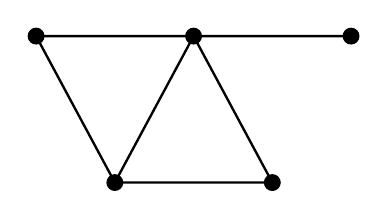
\begin{tikzpicture}
	\draw[line width=0.03cm] (0,0) -- (-1,1.86) -- (1,1.86) -- (0,0) -- (2,0) -- (1,1.86) -- (3,1.86);
	
	\draw[fill=black] (0,0) circle (0.1); 
	\draw[fill=black] (-1,1.86) circle (0.1); 
	\draw[fill=black] (1,1.86) circle (0.1); 
	\draw[fill=black] (2,0) circle (0.1); 
	\draw[fill=black] (3,1.86) circle (0.1); 
	\end{tikzpicture}
	\]



\newpage



% Problem 5
\problem{10} Watch Numberphile's \href{https://www.youtube.com/watch?v=ZCVAGb1ee8A&pp=ygUkUml2ZXIgQ3Jvc3NpbmdzIChhbmQgQWxjdWluIE51bWJlcnMp}{``River Crossings (and Alcuin Numbers)''} on YouTube. Being as detailed as possible, comment on what you learned and how it relates to the course material. 


\end{document}